\subsubsection{Presentation}
Neural Networks (or Multilayer Perceptrons) are a model of supervised learning, represented by composed non-linear functions.\\
\begin{center}
    \captionsetup{type=figure}
    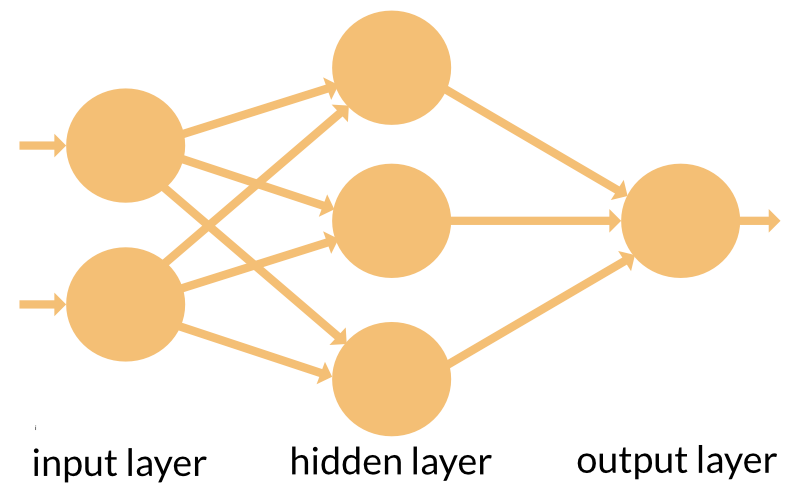
\includegraphics[width=250px]{mlp.png}
    \captionof{figure}{Multilayer Perceptron / Neural Network}\footnote{https://appliedgo.net/perceptron/}
\end{center}
They consist of "neurons", each of which represents a non-linearity, divided in layers, each of which depends on the previous (the first one, on the input data) and is crucial for the next one (the last one gives the output)\\
They can be seen as a function, whose interface is defined by the "input layer" (the first layer) and the "output layer" (the result).\\
All layers between the input layer and the output layer are "hidden layers".\\
A Neural Network makes its predictions after having its parameters (weights) trained with labeled example data (train data)

\subsubsection{Defining Hyperparameters}
The data for training and validating is already defined by the Data Preparation step (80\% train, 20\% validation).\\
Representative hyperparameters (different from the parameters to be trained) for the model are \emph{alpha} and \emph{learning\_rate}
\begin{itemize}
    \item \underline{alpha}: regularization parameter (L2 penalty).
    \item \underline{learning\_rate}: parameter for controlling the step size when updating the weights.
\end{itemize}
A Grid Search is used for getting the best combination of parameters (alpha, learning\_rate) for the input and the model.\\
Values used for \emph{alpha}: [0.001, 0.005, 0.01, 0.05, 0.1]\\
Values used for \emph{learning\_rate}: [0.001, 0.005, 0.01, 0.05, 0.1]
\begin{center}
    \captionsetup{type=figure}
    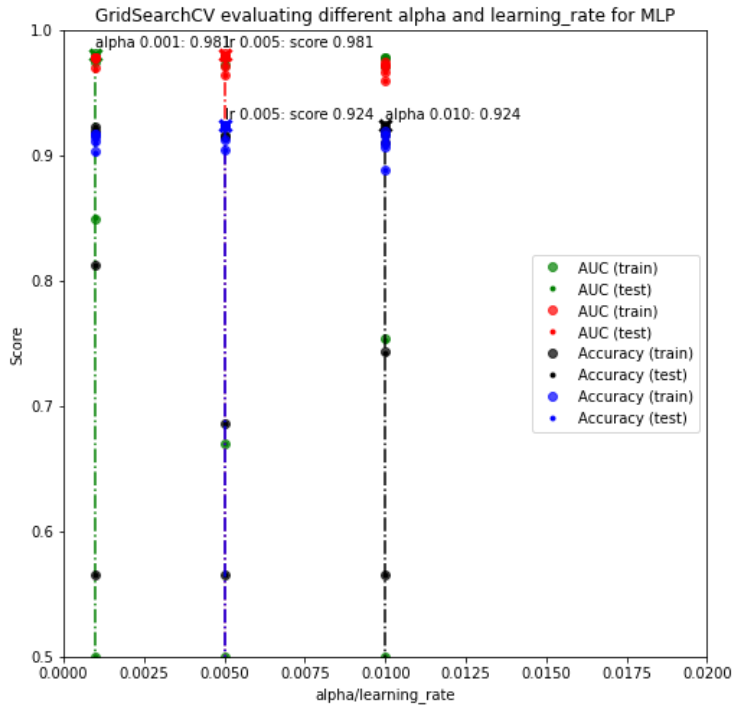
\includegraphics[width=250px]{grid_search_nn.png}
    \captionof{figure}{Grid Search results}
\end{center}
Observable on the plot, and also obtainable by requesting the \emph{grid\_search.best\_params\_}, the best values for the hyperparameters are:
\begin{itemize}
    \item \underline{alpha}: 0.001
    \item \underline{learning\_rate}: 0.005
\end{itemize}

\subsubsection{Model Evaluation}
Chosen the parameters: (\emph{alpha}=0.001, \emph{learning\_rate}=0.005), a learning curve shows us the training and validation scores for different data sizes.\\
This way, we are able to say that the model seems to continue learning after 90000 training rows.
\begin{center}
    \captionsetup{type=figure}
    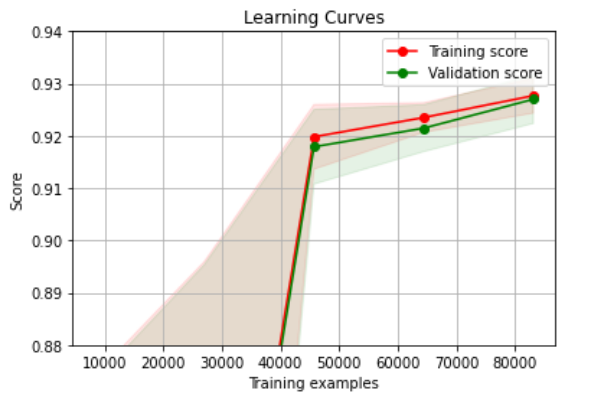
\includegraphics[width=250px]{learning_curve_mlp.png}
    \captionof{figure}{Learning Curve for MLP}
\end{center}
